\chapter[线性基线]{第 2 讲\quad 线性基线：LQR 与它的能力边界}
\label{ch:lqr}

\begin{quote}\small
\textbf{本讲目标}\quad 用最简单的办法把摆"扶住"：在直立点做线性二次型最优控制。
更要紧的是把它的\textbf{能力边界}画出来——吸引域长什么样、全局成功率是多少、
失败是怎么失败的。这条边界会决定后面八讲的全部设计动机。\\[2pt]
\textbf{前置}\quad 第 1 讲的线性化 $A,B$；矩阵求逆与特征值。\\
\textbf{视频}\quad 约 4 分钟。\quad\textbf{代码}\quad \texttt{build/controllers.py}。
\end{quote}

\section{为什么先做线性控制}

第 1 讲已经把难点讲清楚了：非线性、欠驱动、开环不稳定。面对这样的系统，
工程上的第一反应不是"设计一个聪明的非线性控制器"，而是先问：

\begin{quote}
\textbf{在最容易的地方（直立点附近），最好的控制器是什么？它有多好？}
\end{quote}

原因有三个。

\begin{enumerate}[leftmargin=2em,itemsep=3pt]
  \item \textbf{它是最优基准}。在二次型代价下，LQR 是\emph{所有线性反馈}中代价最小的那个。
        任何非线性控制器在局部都不应该比它差——如果差了，说明设计有问题。
  \item \textbf{它是后面所有方法的零件}。第 4 讲的能量整定需要一个"到顶之后接管"的稳定器，
        第 5 讲的滑模需要一个对照，第 6 讲的切换需要一个局部模态。它们用的都是本讲这个东西。
  \item \textbf{它的失败方式最有教学价值}。LQR 不会"慢慢地不行"，它是在某个边界上
        \emph{突然}失效。把这条边界画出来，就知道后面的方法必须补什么。
\end{enumerate}

\section{从 Riccati 方程到增益}

\subsection{问题设定}

线性化模型（第 1 讲式 \eqref{eq:ABnum}）：
\begin{equation}
  \dot{\delta x} = A\,\delta x + B\,\delta u ,
  \qquad \delta x\in\mathbb{R}^4 .
\end{equation}
取二次型代价
\begin{equation}
  J = \int_0^\infty \big(\delta x^\top Q\,\delta x + \delta u^\top R\,\delta u\big)\,dt ,
  \label{eq:cost}
\end{equation}
其中 $Q\succeq 0$ 罚状态偏差、$R\succ 0$ 罚控制量。最优反馈是线性的：
\begin{equation}
  \delta u = -K\,\delta x ,\qquad K = R^{-1}B^\top P ,
  \label{eq:gain}
\end{equation}
其中 $P$ 是\textbf{连续时间代数 Riccati 方程}（CARE）的唯一正定解：
\begin{equation}
  A^\top P + P A - P B R^{-1}B^\top P + Q = 0 .
  \label{eq:care}
\end{equation}

\subsection{本课的具体选择}

\begin{center}
\small
\begin{tabular}{@{}lccl@{}}
\toprule
项 & 取值 & 物理含义 & 为什么这样选 \\
\midrule
$Q_{pp}$ & $1$ & 小车位置 & 权重小：允许车动，只要摆不倒 \\
$Q_{\theta\theta}$ & $40$ & 倾角 & 权重最大：角度是主目标 \\
$Q_{\dot p\dot p}$ & $1$ & 车速 & 抑制来回冲撞 \\
$Q_{\dot\theta\dot\theta}$ & $2$ & 角速度 & 抑制旋转 \\
$R$ & $0.05$ & 力的价格 & 相当于"1\,N$^2$ 值 0.05 的状态代价" \\
\bottomrule
\end{tabular}
\end{center}

把 $A,B,Q,R$ 代入 \eqref{eq:care} 解得 $P$，再算 \eqref{eq:gain}，得到

\begin{empheq}[box=\fbox]{align}
  K &= \begin{bmatrix} -4.4721 & -62.8879 & -9.3145 & -16.4020\end{bmatrix}
  \label{eq:K}\\[2pt]
  \text{闭环极点} &= \{-11.96,\ -4.43,\ -0.902\pm0.47j\}
  \label{eq:poles}
\end{empheq}

四个极点全在左半平面，其中一对共轭复极点 $\sigma\pm j\omega_d$ 给出阻尼比
\begin{equation}
  \zeta = \frac{|\sigma|}{\sqrt{\sigma^2+\omega_d^2}} = 0.89 ,
\end{equation}
也就是说：\textbf{快、但不过冲得太厉害}——这正是重罚角度、轻罚力的结果。

\subsection{增益的直觉}

把 $K$ 的四个分量对着看，物理意义一目了然：

\begin{center}
\small
\begin{tabular}{@{}clp{8.2cm}@{}}
\toprule
分量 & 数值 & 它在说什么 \\
\midrule
$K_p$ & $-4.47$ & 车偏右 $1$\,m，就往左推 $4.47$\,N（慢，位置不重要）\\
$K_\theta$ & $-62.89$ & 摆右倾 $1$\,rad，就往右推 $62.9$\,N（快，角度最要紧）\\
$K_{\dot p}$ & $-9.31$ & 车向右跑，先给一点反向阻力（阻尼）\\
$K_{\dot\theta}$ & $-16.40$ & 摆正在向右倒，提前加大推力（预测/阻尼）\\
\bottomrule
\end{tabular}
\end{center}

\keypoint{$K_\theta/K_p\approx14$ 说明这个控制器"几乎不管车在哪，只管摆的角度"。
这条比例关系会在第 6 讲变成一个具体的坏消息：加了持续侧风之后，
不管位置就意味着车会被慢慢推走。}

\section{局部表现有多好}

数值实验（$\Delta t=20$\,ms，$u$ 限幅 $\pm12$\,N）：

\begin{center}
\small
\begin{tabular}{@{}cccccc@{}}
\toprule
初值 $\theta_0$ & 进入 $\pm0.02$\,rad 用时 & 峰值力 & 饱和时间占比 & 末端 $|p|$ \\
\midrule
$0.10$\,rad & $0.24$\,s & $6.29$\,N & $0\%$ & $0.00$\,m \\
$0.25$\,rad & $1.36$\,s & $12.00$\,N & $1.0\%$ & $0.01$\,m \\
$0.50$\,rad & $1.58$\,s & $12.00$\,N & $4.0\%$ & $0.04$\,m \\
\bottomrule
\end{tabular}
\end{center}

\begin{figure}[htbp]
\centering
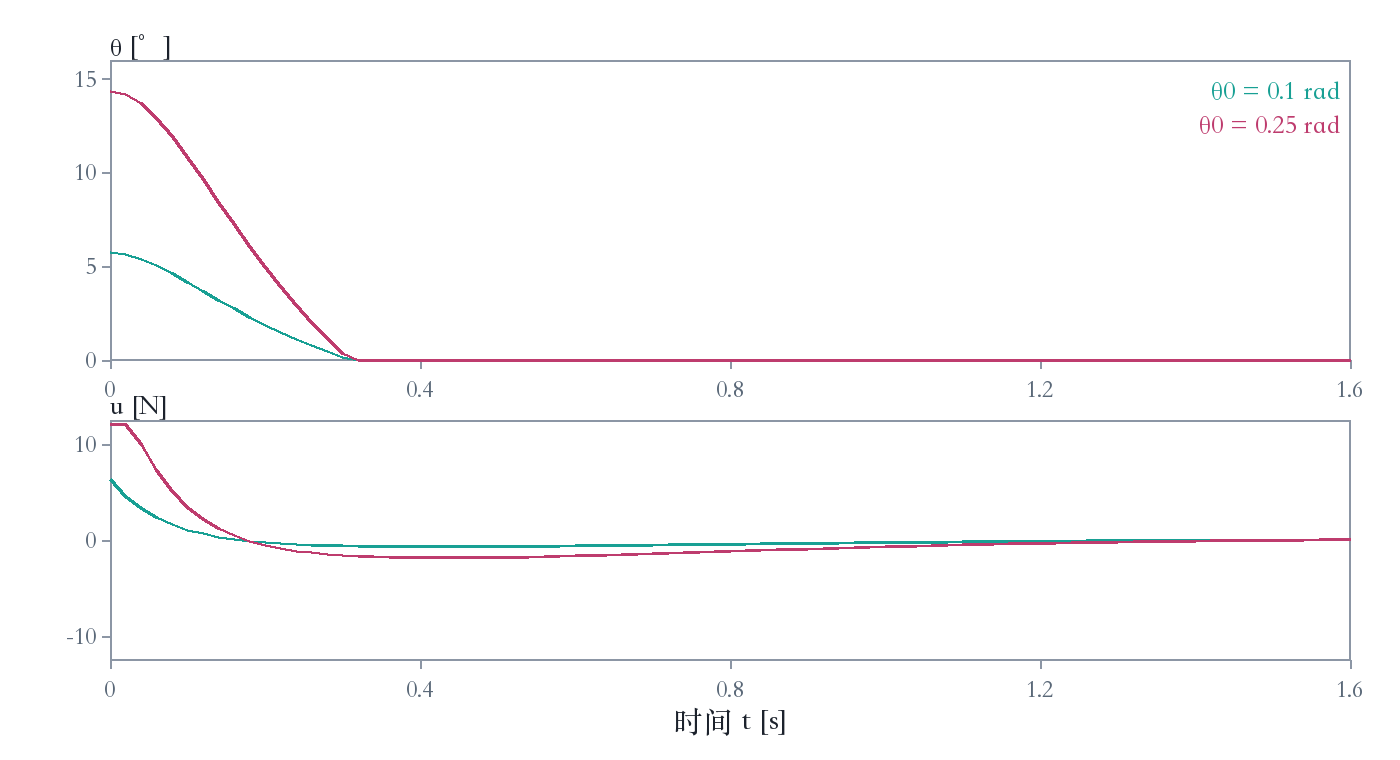
\includegraphics[width=0.92\linewidth]{figures/response.png}
\caption{两个初始角度下的闭环响应：上图为倾角 $\theta(t)$，下图为控制力 $u(t)$。
$0.1$\,rad 出发时峰值力只有 $6.3$\,N；$0.25$\,rad 时开始触及 $12$\,N 限幅，
之后收敛明显变慢（$0.24$\,s $\to$ $1.36$\,s）。\textbf{执行器饱和是第一个真正的非线性}。}
\label{fig:response}
\end{figure}

这里有一个容易被忽略的细节：$0.1$\,rad 到 $0.25$\,rad，初值只大了 $2.5$ 倍，
收敛时间却从 $0.24$\,s 涨到 $1.36$\,s——\textbf{涨了 5.7 倍}。
原因不是"LQR 变差了"，而是力被限幅截断，线性最优解在饱和之后就失效了。
线性控制理论的一切结论都建立在"$u$ 不受限"上。

\section{吸引域：把"局部"画出来}

\subsection{定义与算法}

\begin{quote}
\textbf{吸引域}（region of attraction）：所有能让闭环系统收敛到直立平衡点的初值集合。
\end{quote}

三维状态没法直接画，于是固定 $p_0=\dot p_0=0$，在 $(\theta_0,\dot\theta_0)$ 平面上扫描：

\begin{enumerate}[leftmargin=2em,itemsep=2pt]
  \item 网格：$\theta_0\in[-1.2,1.2]$（61 点）$\times$ $\dot\theta_0\in[-4,4]$（81 点）；
  \item 每个点跑 $3$\,s 闭环仿真；
  \item 判据：过程不撞墙，且末端 $|\theta|<0.05$\,rad、$|p|<1.5$\,m。
\end{enumerate}

共 $61\times81=4941$ 次仿真，结果见图 \ref{fig:basin}。

\begin{figure}[htbp]
\centering
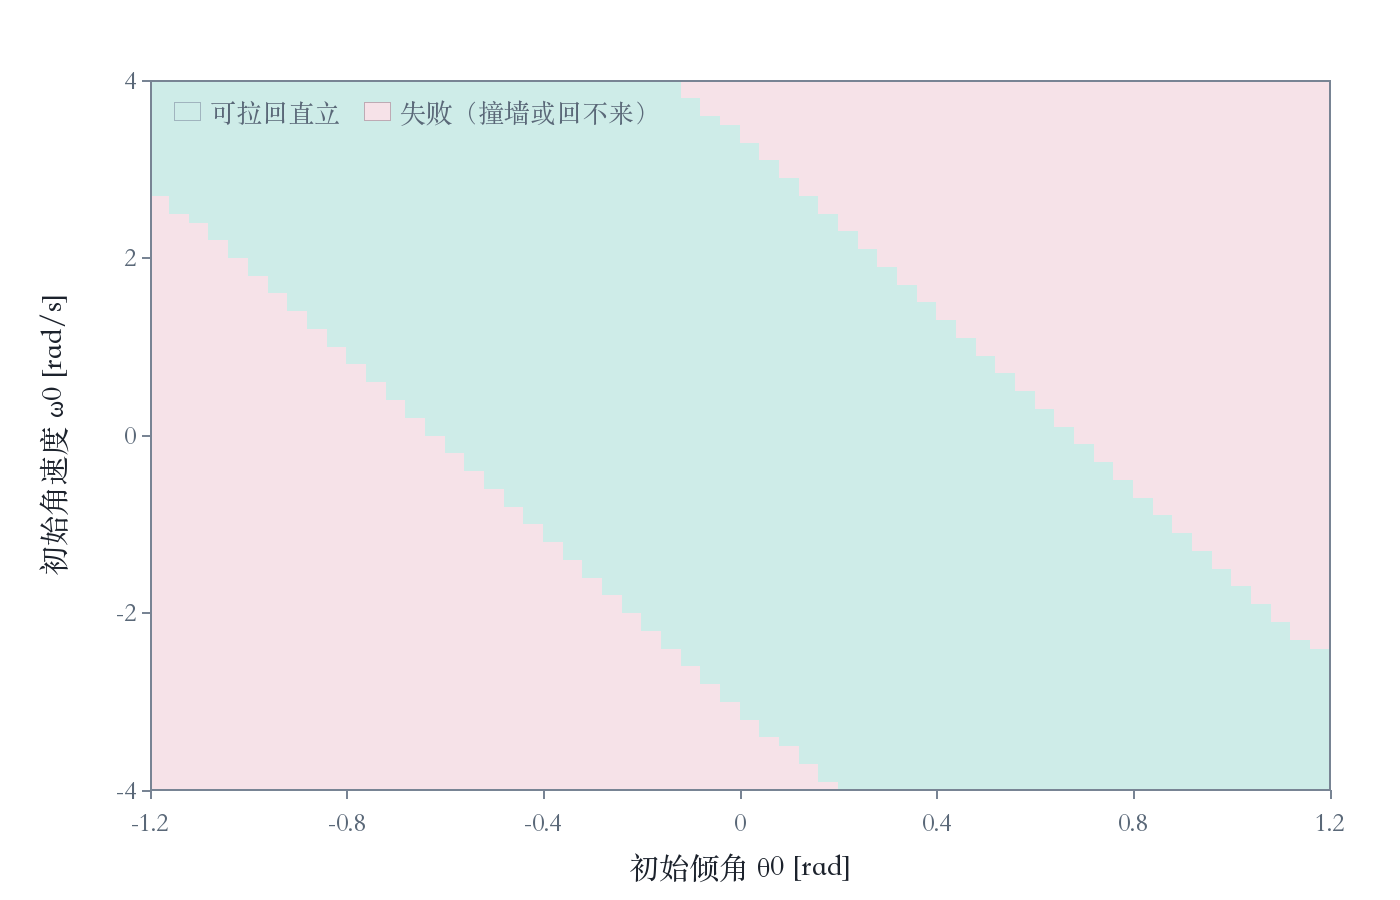
\includegraphics[width=0.86\linewidth]{figures/basin.png}
\caption{LQR 的吸引域。浅色区域能从该初值拉回直立，深色区域失败。
边界不是圆，而是一条\textbf{斜带}：同样大的倾角，如果摆正在朝直立方向转
（$\theta_0>0,\dot\theta_0<0$），容错就大得多。整体关于原点严格点对称
（$4941$ 个格子中 $0$ 个不对称），这来自被控对象的对称性。}
\label{fig:basin}
\end{figure}

\subsection{读图}

\begin{itemize}[leftmargin=2em,itemsep=3pt]
  \item \textbf{面积}：成功区域占整个扫描矩形的 $51.8\%$。
  \item \textbf{静止释放的极限}：$\dot\theta_0=0$ 时，能救回的最大倾角是 $\theta_{\max}=0.64$\,rad
        （约 $37^\circ$）。超过这个角度，无论怎么推都来不及。
  \item \textbf{斜带}：在 $\dot\theta_0=-4$\,rad/s（快速朝直立方向转）时，$\theta_0$ 可以大到 $1.2$\,rad；
        反过来，如果摆正在\textbf{远离}直立的方向快速旋转，能救的范围就小得多。
  \item \textbf{点对称}：把图旋转 $180^\circ$ 与自身完全重合。这说明边界是被控对象的性质，
        不是控制器或仿真器的缺陷。
\end{itemize}

\section{全局失败：$25\%$ 与 $82\%$}

把同一份参数丢到"真实任务"里：$60$ 组随机初值（$\theta_0$ 在整圈上均匀分布、$p_0\in\pm1$\,m），
$12$\,s 闭环，成功判据同第 1 讲。

\begin{center}
\small
\begin{tabular}{@{}lcc@{}}
\toprule
指标 & LQR（本讲） & 说明 \\
\midrule
成功率 & $25\%$ & 只有四分之一的初值能被救回来 \\
撞墙率 & $82\%$ & 绝大多数回合把车推到导轨尽头 \\
末端 $|\theta|$ 均值 & $1.62$\,rad & 失败回合基本是"躺平"或"乱转" \\
平均 $|p|_{\max}$ & $2.17$\,m & 几乎贴着 $2.4$\,m 的导轨极限 \\
\bottomrule
\end{tabular}
\end{center}

\subsection{失败是怎么发生的}

从下垂位置（$\theta_0=\pi-0.1$）出发，LQR 的行为可以逐秒复述：

\begin{enumerate}[leftmargin=2em,itemsep=2pt]
  \item $0$--$0.3$\,s：$\theta\approx\pi$，$K_\theta\theta\approx-191$\,N 远超限幅，
        于是 $u=+12$\,N 立刻饱和（推力朝右，因为在本讲约定里 $\theta>0$ 表示"摆向右倾"）；
  \item $0.3$--$1.5$\,s：车被推向右侧极限，摆杆因为小车加速而略有摆动，
        但幅度远不足以翻上来；
  \item 之后：车撞墙（位置钳位、速度清零），摆继续倒下或乱转，控制量来回打满。
\end{enumerate}

\keypoint{LQR 的失败不是因为"参数没调好"，而是因为它在 $\theta\approx\pi$ 处的
\textbf{线性化模型完全错了}：第 1 讲已经量化过，$1$\,s 后线性化预测与实际相差 $35\%$，
更何况 $\pm\pi$ 附近 $\sin\theta\approx\theta$ 的假设早已失效。
换句话说——\textbf{它在用一个错误的地图全力导航}。}

\subsection{一个反直觉的现象}

当 $\theta$ 接近 $\pi$ 时，$K_\theta\cdot\theta$ 这一项会给出巨大的力
（$62.89\times3.14\approx197$\,N，远超 $12$\,N 限幅），所以控制器\textbf{永远处于饱和}。
饱和之后，闭环就退化成"恒定 $-12$\,N 的开环推力"，摆当然不会立起来。
这解释了一个常见误解：\emph{以为换个更好的 $Q,R$ 就能全局收敛}。
实际上表 \ref{tab:designs} 会看到，增大增益只会让饱和更早发生，吸引域几乎不变。

\section{$Q/R$ 怎么选：三组设计的对比}

\begin{center}
\small
\begin{tabular}{@{}lcccccc@{}}
\toprule
设计 & $Q$ & $R$ & $K_\theta$ & 收敛时间 & 峰值力 & 吸引域占比 \\
\midrule
温和 & $\mathrm{diag}(1,10,0.3,0.5)$ & $1.0$ & $-27.5$ & $1.96$\,s & $12$\,N & $37\%$ \\
默认 & $\mathrm{diag}(1,40,1,2)$ & $0.05$ & $-62.9$ & $1.36$\,s & $12$\,N & $52\%$ \\
激进 & $\mathrm{diag}(1,120,3,5)$ & $0.01$ & $-178.5$ & $1.36$\,s & $12$\,N & $52\%$ \\
\bottomrule
\end{tabular}
\captionof{table}{三组 $Q/R$ 的对比（$\theta_0=0.25$\,rad 出发）。}
\label{tab:designs}
\end{center}

读这张表有两个结论：

\begin{enumerate}[leftmargin=2em,itemsep=2pt]
  \item \textbf{$Q/R$ 决定"多激进"，不决定"能走多远"}。温和→默认，收敛时间从 $1.96$\,s
        降到 $1.36$\,s，吸引域从 $37\%$ 涨到 $52\%$；但默认→激进，两个指标\textbf{都不再改善}。
  \item \textbf{天花板是执行器}。激进设计把 $K_\theta$ 从 $63$ 提到 $179$，但峰值力早就顶到 $12$\,N，
        更高的增益只是让饱和更早、更久。\textbf{在饱和世界里，增益不是免费的。}
\end{enumerate}

\keypoint{这一节给出了本讲的中心结论：\textbf{局部最优 ≠ 全局可行}。
在一个 $25\%$ 成功率的世界里，把一个 $0.64$\,rad 的吸引域再优化 $20\%$ 没有意义；
真正缺的是"从头到尾"的策略——那就需要第 4 讲的能量、第 6 讲的切换。}

\section{从失败读出设计需求}

把上面的观察翻译成三条设计需求，正好对应后面三讲：

\begin{center}
\small
\begin{tabular}{@{}lp{4.4cm}p{4.4cm}@{}}
\toprule
观察 & 需求 & 对应讲 \\
\midrule
$\theta$ 大时线性模型失效 & 需要一个不依赖小角假设的全局控制律 & 第 4 讲（能量整定）\\
饱和让"更强的反馈"失效 & 需要主动管理能量而不是被动加增益 & 第 4、5 讲 \\
没有位置积分、抗扰差 & 需要把鲁棒性写进结构 & 第 5 讲（滑模）\\
两个目标（位置/角度）争一个输入 & 需要按状态分区、显式切换 & 第 6 讲（监督器）\\
\bottomrule
\end{tabular}
\end{center}

\section{本讲小结}

\begin{enumerate}[leftmargin=2em,itemsep=2pt]
  \item LQR 通过解 CARE 得到最优线性反馈：$K=[-4.47,-62.89,-9.31,-16.40]$，
        闭环极点 $\{-11.96,-4.43,-0.90\pm0.47j\}$，阻尼比 $0.89$。
  \item 局部表现极好：$0.1$\,rad 出发 $0.24$\,s 进入 $\pm0.02$\,rad，峰值力只有 $6.3$\,N。
  \item 吸引域是一条\textbf{斜带}：静止释放的极限倾角 $0.64$\,rad，面积占比 $51.8\%$，
        关于原点严格点对称。
  \item 全局失败：$25\%$ 成功率、$82\%$ 撞墙率。失败根源是\textbf{线性化在地图之外失效}
        加上\textbf{力被限幅}，而不是参数没调好。
  \item $Q/R$ 只能调"多激进"，调不动"能走多远"；天花板由执行器决定。
\end{enumerate}

\section*{习题}
\addcontentsline{toc}{section}{习题}

\begin{enumerate}[leftmargin=2em,itemsep=6pt]
  \item 手算验证 $K_\theta/K_p\approx 14$ 的由来：从 CARE 出发，解释为什么重罚 $\theta$
        会让这两个分量的比例变大。
  \item 把 $R$ 从 $0.05$ 调到 $0.5$，重算 $K$ 与闭环极点，并解释阻尼比的变化方向。
  \item 只用 $p,\theta$ 两个状态（去掉速度反馈，即 $K_{\dot p}=K_{\dot\theta}=0$）
        重新设计，看吸引域缩小多少，并解释原因。
  \item 让 $u_{\max}$ 从 $12$\,N 增加到 $20$\,N，重跑吸引域扫描：面积占比变成多少？
        这说明"能力边界"主要由什么决定？
  \item 在 $\theta_0=0.6$\,rad、$\dot\theta_0=0$ 的边界附近，画出 $\theta(t)$ 的相图，
        观察它是"刚好回来"还是"擦边失败"。
  \item （编程）复现 \S2.4 的吸引域扫描，并把判据从"$3$\,s 内收敛"改成"$6$\,s 内收敛"，
        看边界变化多少。这个敏感性说明了什么？
\end{enumerate}

\section*{延伸阅读}
\addcontentsline{toc}{section}{延伸阅读}
\begin{itemize}[leftmargin=2em,itemsep=2pt]
  \item B. D. O. Anderson, J. B. Moore, \emph{Optimal Control: Linear Quadratic Methods},
        Dover, 2007.（CARE 的完整推导与数值解法）
  \item R. Tedrake, \emph{Underactuated Robotics}, 第 8 章：LQR 与轨迹优化。
  \item 关于吸引域的计算：E. Najafi et al., \emph{Computing the region of attraction...},
        CDC 2016（平方和规划与网格法的对比）。
\end{itemize}
